\documentclass[fontsize=14pt,DIV=1,a4paper]{scrartcl} 
\usepackage[utf8]{inputenc}
\usepackage{cmap} % для кодировки шрифтов в pdf
\usepackage[T2A]{fontenc}
%\usepackage{fontspec}
%\usepackage{polyglossia}
%\setmainfont{Times New Roman}
%\newfontfamily\cyrillicfont{Times New Roman}
%\usepackage{mathptmx}
%\renewcommand{\rmdefault}{ftm} % Times New Roman
\linespread{1.3} % полуторный интервал
\frenchspacing
\usepackage[english,russian,ukrainian]{babel}
\usepackage{indentfirst}
\usepackage{misccorr}
\usepackage{graphicx}
\usepackage[left=3cm,right=1.5cm,top=2cm,bottom=2cm,includefoot]{geometry}
\usepackage{graphicx}% для вставки картинок
\graphicspath{ {/home/zeka/Documents/lab2chmmph/} }

\usepackage{amssymb,amsfonts,amsmath,amsthm} % математические дополнения от АМС
\usepackage{indentfirst} % отделять первую строку раздела абзацным отступом тоже
\usepackage[usenames,dvipsnames]{color} % названия цветов
\usepackage{makecell}
\usepackage{multirow} % улучшенное форматирование таблиц
\usepackage{ulem} % подчеркивания
\usepackage{gensymb}
\usepackage{hyperref}
\hypersetup{
    colorlinks=true,
    linkcolor=black,
    filecolor=black,      
    urlcolor=black,
}

\makeatletter
\DeclareOldFontCommand{\rm}{\normalfont\rmfamily}{\mathrm}
\DeclareOldFontCommand{\sf}{\normalfont\sffamily}{\mathsf}
\DeclareOldFontCommand{\tt}{\normalfont\ttfamily}{\mathtt}
\DeclareOldFontCommand{\bf}{\normalfont\bfseries}{\mathbf}
\DeclareOldFontCommand{\it}{\normalfont\itshape}{\mathit}
\DeclareOldFontCommand{\sl}{\normalfont\slshape}{\@nomath\sl}
\DeclareOldFontCommand{\sc}{\normalfont\scshape}{\@nomath\sc}
\makeatother

\begin{document}
	\begin{titlepage}
		\begin{center}
			\large
			\textbf{КИЇВСЬКИЙ НАЦІОНАЛЬНИЙ УНІВЕРСИТЕТ \\
			ІМЕНІ ТАРАСА ШЕВЧЕНКА}

			\textbf{Кафедра обчислювальної математики}
			
			\vspace{6.0cm}

			\textsc{Лабораторна робота 3}\\
			На тему:

			\textbf{ Вирішення задач теплопровідності }
			\bigskip
		\end{center}
		\vfill

		\hfill
		\begin{minipage}{0.6\textwidth}
			студента 4-го курсу бакалаврату\\
			Гаврилка Євгенія Дмитровича
		\end{minipage}%
		\vfill
		
		\vspace{-2.5cm}
		
		

		\vspace{1.0cm}

		\begin{center}
			Київ – 2017
		\end{center}
	\end{titlepage}
	
	\tableofcontents

	%summary
	\newpage
	\addcontentsline{toc}{section}{Постанова задачі}
	\section*{Постанова задачі}
	Визначити температуру всередині і на повурхні цегляної колони діметром 0.5 м через одну годину, якщо раптово температура навколишнього середовища знизилась з +20 до - 20 С. Фізичні характеристики цегляної колони мають такі значення: $\lambda = 0.77\quad W/(m \cdot K); c= 0.83\quad kJ/(kg \cdot K); \rho = 1600 \quad kg/m^3ну ; \gamma = 7 \quad W/(m^2 \cdot K) $
	\begin{figure}[h!]
		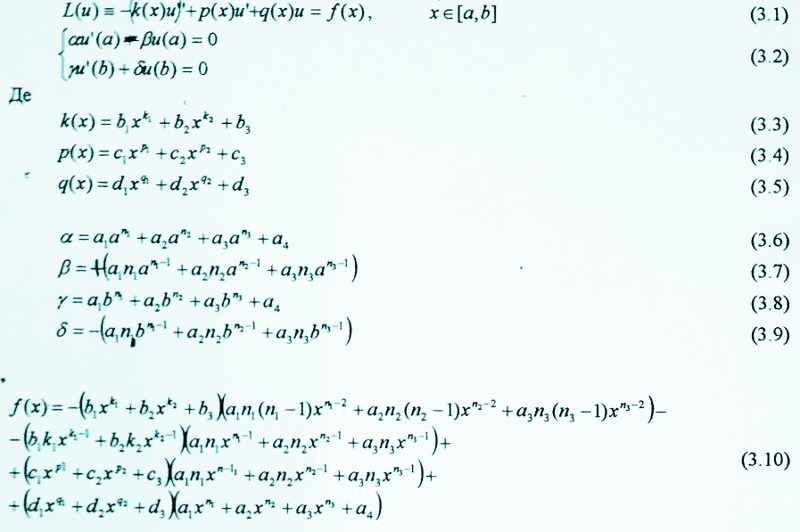
\includegraphics[scale=0.5]{stand.png}
		\centering
	\end{figure}
	
	%section1
	\newpage
	\section{Iнтего-інтерполяційним метод}
	\subsection{Теорія}
	Розглядається задача Au=f з крайовими умовами. Головна ідея полягає в тому що б протабулювати значення функції на сітці. Крайові рівняння обирається так, щоб задовольняти крайовим умовам. Тобто
	\begin{figure}[h!]
		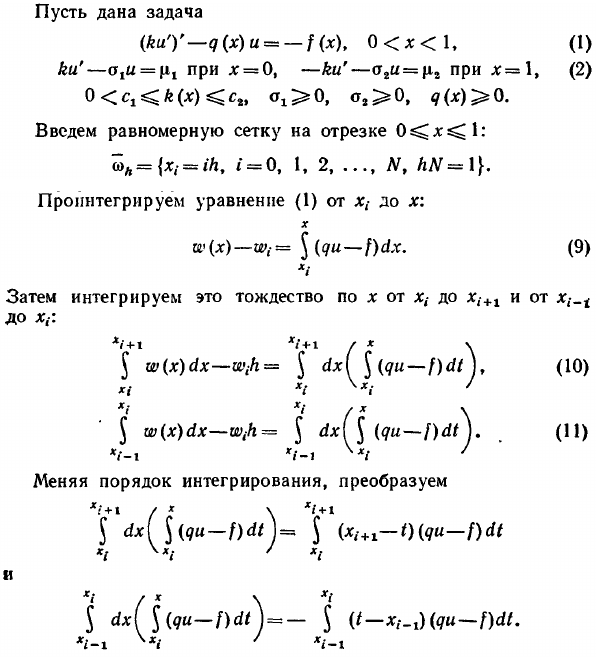
\includegraphics[scale=0.6]{iim_th1.png}
		\centering
		\caption{Теорія}
	\end{figure}
	
	\begin{figure}[h!]
		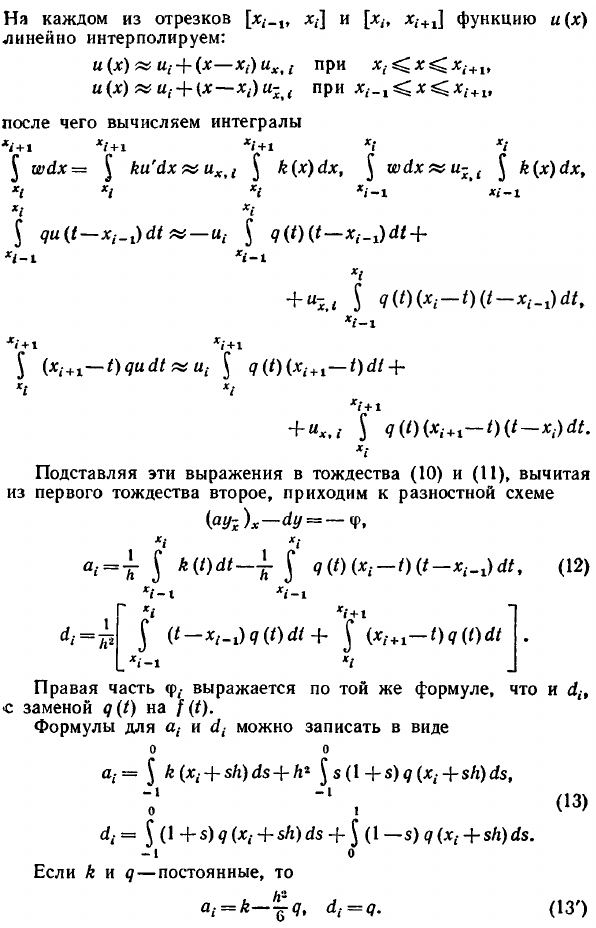
\includegraphics[scale=0.6]{iim_th2.png}
		\centering
		\caption{Теорія}
	\end{figure}
	
	\newpage
	\textbf{}
			
	\newpage
	\subsection{Алгоритм}
	
	\begin{figure}[h!]
		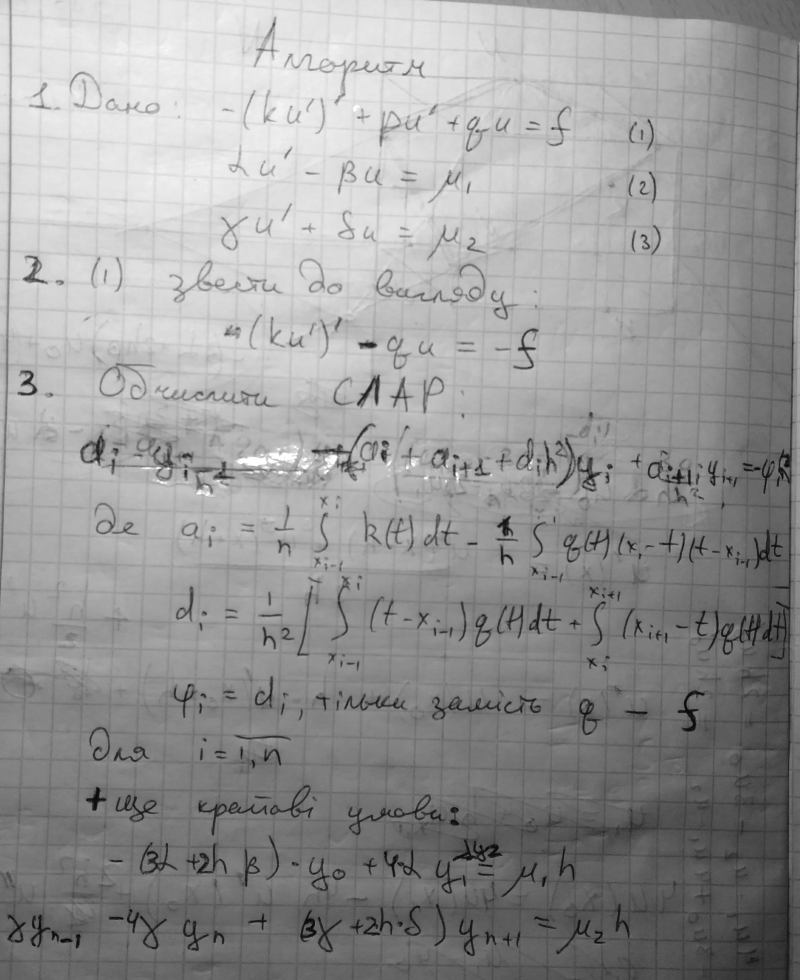
\includegraphics[scale=0.5]{algo.png}
		\centering
		\caption{Алгоритм}
	\end{figure}
	
	\newpage
	\section{Практична частина}
	
    \vspace{10px}
    n = 10
    \vspace{10px}

    \begin{tabular}{| c | c | c | c | c |}
        \hline
        x & u & y & $\delta_y$ & $\varepsilon_y$ \\
        \hline
        1.00 &   12.00 &    7.02 &    4.9767 &   41.4724\% \\
        1.27 &   17.55 &   11.18 &    6.3733 &   36.3077\% \\
        1.55 &   27.38 &   18.86 &    8.5179 &   31.1094\% \\
        1.82 &   44.16 &   32.56 &   11.6018 &   26.2703\% \\
        2.09 &   71.61 &   55.73 &   15.8833 &   22.1801\% \\
        2.36 &  114.64 &   92.93 &   21.7060 &   18.9343\% \\
        2.64 &  179.55 &  150.03 &   29.5216 &   16.4419\% \\
        2.91 &  274.22 &  234.30 &   39.9198 &   14.5575\% \\
        3.18 &  408.27 &  354.60 &   53.6672 &   13.1450\% \\
        3.45 &  593.26 &  521.50 &   71.7570 &   12.0954\% \\
        3.73 &  842.85 &  747.37 &   95.4747 &   11.3276\% \\
        4.00 & 1173.00 & 1046.52 &  126.4825 &   10.7828\% \\
        \hline
    \end{tabular}

    \vspace{10px}
    n = 100
    \vspace{10px}

    \begin{tabular}{| c | c | c | c | c |}
        \hline
        x & u & y & $\delta_y$ & $\varepsilon_y$ \\
        \hline
        1.00 &   12.00 &   11.93 &    0.0681 &    0.5677\% \\
        1.30 &   18.22 &   18.13 &    0.0924 &    0.5071\% \\
        1.59 &   29.77 &   29.64 &    0.1298 &    0.4360\% \\
        1.89 &   50.28 &   50.09 &    0.1842 &    0.3664\% \\
        2.19 &   84.86 &   84.60 &    0.2611 &    0.3076\% \\
        2.49 &  140.43 &  140.06 &    0.3676 &    0.2618\% \\
        2.78 &  225.90 &  225.38 &    0.5136 &    0.2273\% \\
        3.08 &  352.53 &  351.81 &    0.7119 &    0.2019\% \\
        3.38 &  534.17 &  533.19 &    0.9799 &    0.1834\% \\
        3.67 &  787.57 &  786.23 &    1.3402 &    0.1702\% \\
        3.97 & 1132.59 & 1130.77 &    1.8232 &    0.1610\% \\
        \hline
    \end{tabular}
    
    \vspace{10px}
    n = 1000
    \vspace{10px}

    \begin{tabular}{| c | c | c | c | c |}
        \hline
        x & u & y & $\delta_y$ & $\varepsilon_y$ \\
        \hline
        1.00 &   12.00 &   12.00 &    0.0007 &    0.0058\% \\
        1.30 &   18.30 &   18.30 &    0.0010 &    0.0052\% \\
        1.60 &   30.05 &   30.05 &    0.0013 &    0.0045\% \\
        1.90 &   51.00 &   51.00 &    0.0019 &    0.0038\% \\
        2.20 &   86.45 &   86.45 &    0.0027 &    0.0032\% \\
        2.50 &  143.55 &  143.55 &    0.0038 &    0.0027\% \\
        2.80 &  231.56 &  231.56 &    0.0054 &    0.0023\% \\
        3.10 &  362.18 &  362.17 &    0.0075 &    0.0021\% \\
        3.40 &  549.79 &  549.78 &    0.0103 &    0.0019\% \\
        3.70 &  811.79 &  811.78 &    0.0142 &    0.0017\% \\
        4.00 & 1168.87 & 1168.85 &    0.0193 &    0.0017\% \\
        \hline
    \end{tabular}

%	\begin{figure}[h!]
%		\includegraphics[scale=0.5]{plot2.png}
%		\centering
%		\caption{n=2}
%	\end{figure}
	
	%results
	\newpage
	\addcontentsline{toc}{section}{Висновки}
	\section*{Висновки}
	
	Як видно з результатів, метод дійсно має точність $h^2$. Але для її досягнення необхідно брати з відповідною апроксимацією і різнецеву схему, і крайові умови.

\end{document}
